\section{Stokes' Flow with Odd Viscosity}

\emph{(Guest lecture by Tali Khain)}

Today, we'll discuss the Stokes' fluid flow problem around a sphere, first reviewing the problem for a normal fluid, then studying what happens when we add odd viscosity.

\subsection{The Stokeslet}
We consider the Reynold's number:
\begin{equation}
    \text{Re} = \frac{\rho U L}{\mu}
\end{equation}
which is low, e.g., when we look at small particles travelling in a fluid (as $L$ in this case is small). In this scenario, the Navier-Stokes equation reduces to:
\begin{equation}
    -\nabla p + \mu \nabla^2 \v{v} = -\v{F}(\v{r})
\end{equation}
and we also assume that the fluid is incompressible:
\begin{equation}
    \nabla \cdot \v{v} = 0
\end{equation}
Since these equations are linear in $p, \v{v}$, analytical progress is possible. 

We can make an analogy with electrostatics, where we have the Poisson equation:
\begin{equation}
    \nabla^2 \phi = 4\pi \rho(\v{r})
\end{equation}
The first problem we solve is that for a point charge, where we have the Green's function solution:
\begin{equation}
    \nabla^2 G = q\delta^3(\v{r})
\end{equation}
which is the first order/monopole term in the multiple expansion when looking for the potential $\phi(\v{r})$ of an arbitrary charge distribution $\rho(\v{r})$.

The analogy we make is charge $\leftrightarrow$ forces, potential $\leftrightarrow $ velocity. Today, we compute the Green's function of the Stoke's equations, which tells us the response of a fluid to a point force.

\begin{center}
    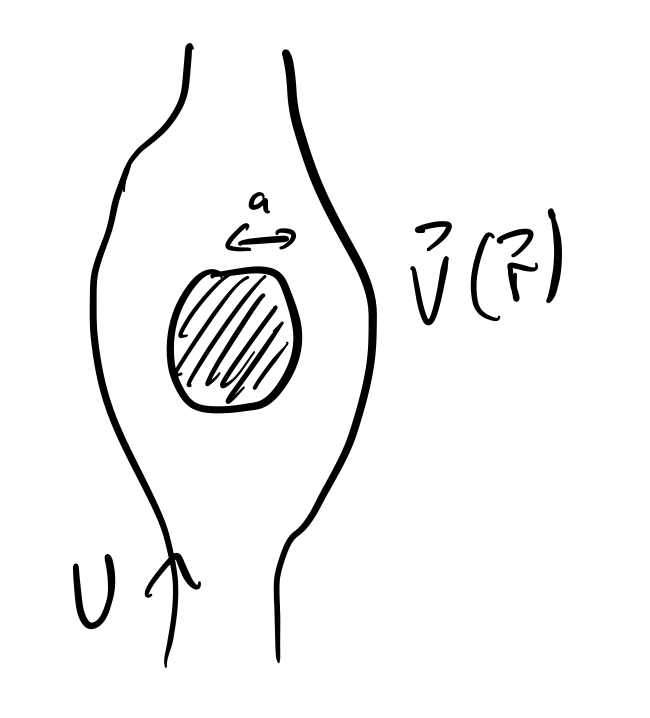
\includegraphics[scale=0.35]{Lectures/Images/lec12-sphereinfluid.png}
\end{center}

A common problem we study in fluid mechanics is we study a spherical particle in a medium, under force $\v{F}$ and fluid velocity field $\v{v}$. We work in the overdamped regime, where $F \sim U$. The stokes drag is then given as:
\begin{equation}
    U \sim \frac{F}{6\pi \mu a}
\end{equation}
with $a$ the length scale of the sphere. The velocity field is given by:
\begin{equation}
    \v{v} = \frac{\v{F}}{8\pi\mu}\cdot (1 + \frac{a^2}{6}\nabla^2)\mathbb{G}
\end{equation}
in the regime of small $a$ we can neglect the $\nabla^2$ term, so:
\begin{equation}
    \v{v} = \frac{\v{F}}{8\pi\mu}\cdot \mathbb{G}
\end{equation}
we can interpret this as like solving for the ``monopole'' term/far field limit in electrostatics. This primary Green's function is what is known as the Stokeslet.

\subsection{Solving Navier-Stokes with Point Flow Source}
We solve the equations:
\begin{equation}
    -\nabla p + \mu \nabla^2 \v{v} = -\v{F}\delta^3(\v{r})
\end{equation}
\begin{equation}
    \nabla \cdot \v{v} = 0
\end{equation}
by going into fourier space; we have the Fourier and inverse Fourier transforms:
\begin{equation}
    f(\v{k}) = \int d^3\v{r}f(\v{r})e^{-i\v{k}\cdot\v{r}}
\end{equation}
\begin{equation}
    f(\v{r}) = \frac{1}{(2\pi)^3}\int d^3\v{k}f(\v{k})e^{i\v{k} \cdot \v{r}}
\end{equation}
so then $\nabla \to i\v{k}$ in Fourier space. In $\v{k}$-space the equations become:
\begin{equation}
    -i\v{k}p - \mu k^2\v{v} = -\v{F}
\end{equation}
\begin{equation}
    \v{k} \cdot \v{v} = 0
\end{equation}
to eliminate the velocity term, we apply $\v{k} \cdot$ to the first equation, which yields:
\begin{equation}
    -ik^2p - \mu k^2 \v{k} \cdot \v{v} = -\v{k} \cdot \v{F} \implies -k^2p = -\v{k} \cdot \v{F} \implies p = -i\frac{\v{k}\cdot\v{F}}{k^2}
\end{equation}
Plugging back in this expression for the pressure to solve for the velocity:
\begin{equation}
    -i\v{k}\left(-i\frac{\v{k}\cdot\v{F}}{k^2}\right) - \mu k^2\v{v} = -\v{F} \implies \v{v} = \frac{1}{\mu k^2}\left[\v{F} - \v{k}\left(\frac{\v{k} \cdot \v{F}}{k^2}\right)\right] = \frac{1}{\mu k^2}\left[\II - \frac{\v{k} \v{k}}{k^2}\right]\cdot \v{F}
\end{equation}
where $\v{k}\v{k}$ is the matrix $(\v{k}\v{k})_{ij} = k_ik_j$. Our Green's function in Fourier space is therefore:
\begin{equation}
    \mathbb{G}(\v{k}) = \frac{1}{\mu k^2}\left[\II - \frac{\v{k} \v{k}}{k^2}\right]
\end{equation}
And our velocity field in position space is obtained by taking the inverse Fourier transform:
\begin{equation}\label{eq:intermediatev}
    \v{v}(\v{r}) = \frac{1}{(2\pi)^3}\int d^3\v{k}\frac{1}{\mu k^2}\left[\II - \frac{\v{k}\v{k}}{k^2}\right]\cdot\v{F}e^{i\v{k} \cdot \v{r}}
\end{equation}
This is the tricky part - going back to real space. Formally, we solve these by contour integration in the complex plane. But, for this class we will take a few shortcuts and use results that you may know already. From electrostatics, recall:
\begin{equation}
    \nabla^2 \phi = -\delta^3(\v{r})
\end{equation}
\begin{equation}
    \phi(\v{r}) = \frac{1}{4\pi r} = \frac{1}{(2\pi)^3}\int d^3\v{k} \frac{1}{k^2}e^{i\v{k} \cdot \v{r}}
\end{equation}
from which:
\begin{equation}
    -k^2\phi = -1 \implies \phi = \frac{1}{k^2}
\end{equation}
This gives us the first term. The analogous process for the biharmonic equation is:
\begin{equation}
    \nabla^4 \psi(\v{r}) = -\delta^3(\v{r})
\end{equation}
so:
\begin{equation}
    \psi(\v{r}) = \frac{r}{8\pi}
\end{equation}
so then:
\begin{equation}
    k^4\psi = -1 \implies \psi = -\frac{1}{k^4}
\end{equation}
and so we have the equation:
\begin{equation}
    \psi(\v{r}) = \frac{r}{8\pi} = -\frac{1}{(2\pi)^3}\int d^3k \frac{1}{k^4}e^{i\v{k} \cdot \v{r}}
\end{equation}
but we notice that we don't just require the inverse fourier transform of $\frac{e^{i\v{k} \cdot \v{r}}}{k^4}$ but with the $\v{k}\v{k}$ in the numerator, so we take two derivatives:
\begin{equation}
    \nabla \nabla(\frac{r}{8\pi}) = -\frac{1}{(2\pi)^3}\int d^3k\frac{\v{k}\v{k}}{k^4}e^{i\v{k} \cdot \v{r}}
\end{equation}
But what exactly is the object on the LHS? Well:
\begin{equation}
    \p_i \p_j\left(\frac{r}{8\pi}\right) = \frac{1}{8\pi}\p_i\left(\frac{r_i}{r}\right) = \frac{1}{8\pi}\left[\frac{\delta_{ij}r - \frac{r_i}{r}r_j}{r^2}\right] = \frac{1}{8\pi}\left[\frac{\delta_{ij}}{r} - \frac{r_ir_j}{r^3}\right] = \frac{1}{8\pi}\left[\frac{\II}{r} - \frac{\v{r}\v{r}}{r^3}\right]
\end{equation}

So combining these two results, we can return back to our velocity field integral in Eq. \eqref{eq:intermediatev} to obtain:
\begin{equation}
    \v{v}(\v{r}) = \frac{1}{\mu}\left[\frac{\II}{4\pi r} - \frac{\II}{8\pi r} + \frac{\v{r} \v{r}}{8\pi r^3}\right]\cdot\v{F} = \frac{1}{8\pi \mu r}\left[\II + \frac{\v{r}\v{r}}{r^2}\right]\cdot\v{F}
\end{equation}
we have thus obtained the Green's function in real space:
\begin{equation}
    \mathbb{G}(\v{r}) = \frac{1}{8\pi \mu 4}\left[\II + \frac{\v{r}\v{r}}{r^2}\right]
\end{equation}
and we can also proceed to solve for the pressure $p(\v{r})
$. This is what happens for a normal fluid - what happens when we add odd viscosity?

\subsection{Solving Navier-Stokes with Odd Viscosity}
If we now also have odd viscosity, the first equation of Navier-Stokes is modified to be:
\begin{equation}
    -\nabla p + \m{\mu & \eta^0 & 0 \\ -\eta^0 & \mu & 0 \\ 0 & 0 & \mu}\nabla^2\v{v} = -\v{F}\delta^3(\v{r})
\end{equation}
with the $\eta^0$ term corresponding to the odd viscosity coefficient. We have chosen the rotation axis of the fluid molecules (which gives rise to the odd viscosity) to be $\hat{\v{z}}$ and hence this is why the odd viscosity terms only appear in $xy$, and the above matrix is not isotropic. Defining $\gamma = \frac{\eta^0}{\mu}$, the above equation becomes:
\begin{equation}
    -\nabla p + \mu\m{1 & \gamma & 0 \\ -\gamma & 1 & 0 \\ 0 & 0 & 1}\nabla^2\v{v} = -\nabla p + \mu\mathbb{M}\nabla^2 \v{v} = -\v{F}\delta^3(\v{r})
\end{equation}
Again going into Fourier space:
\begin{equation}\label{eq:fourierodd}
    -i\v{k}p - \mu \mathbb{M}k^2\v{v} = -\v{F}
\end{equation}
\begin{equation}
    \v{k} \cdot \v{v} = 0
\end{equation}
Let us multiply the first equation by $\mathbb{M}^{-1}$:
\begin{equation}
    -i\mathbb{M}^{-1}\v{k}p - \mu k^2 \v{v} = -\mathbb{M}^{-1}\v{F}
\end{equation}
and now multiplying this by $\v{k}\cdot$ to get rid of the velocity term:
\begin{equation}
    -i\v{k} \cdot \mathbb{M}^{-1}\v{k}p = -\v{k}\cdot \mathbb{M}^{-1}\v{F}
\end{equation}
Solving for $p$:
\begin{equation}
    p = -i\frac{\v{k} \cdot \mathbb{M}^{-1}\v{F}}{\v{k} \cdot \mathbb{M}^{-1}\v{k}}
\end{equation}
We can now plug this back into Eq. \eqref{eq:fourierodd} to solve for the velocity:
\begin{equation}
    -\v{k}\frac{\v{k} \cdot \mathbb{M}^{-1}\v{F}}{\v{k} \cdot \mathbb{M}^{-1}\v{k}} - \mu \mathbb{M}k^2\v{v} = -\v{F}
\end{equation}
\begin{equation}
    \v{v} = \frac{1}{\mu k^2}\mathbb{M}^{-1}\left[\v{F} - \v{k}\left(\frac{\v{k} \cdot \mathbb{M}^{-1}\v{F}}{\v{k} \cdot \mathbb{M}^{-1}\v{k}}\right)\right] = \frac{\mathbb{M}^{-1}}{\mu k^2}\left[\II - \frac{\v{k}(\v{k}\cdot \mathbb{M}^{-1})}{\v{k}\cdot(\mathbb{M}^{-1}\v{k})}\right]\cdot\v{F}
\end{equation}
Now, considering the limit $\gamma = \frac{\eta_0}{\mu} \ll 1$, we can write:
\begin{equation}
    \mathbb{M} = \II + \gamma \e
\end{equation}
with:
\begin{equation}
    \e = \m{0 & 1 & 0 \\ -1 & 0 & 0 \\ 0 & 0 & 0}
\end{equation}
where then:
\begin{equation}
    \mathbb{M}^{-1} = \II - \gamma \e
\end{equation}
Then in this small $\gamma$ limit:
\begin{equation}
    \v{k} \cdot \mathbb{M}^{-1}\v{k} = k^2 - \gamma \v{k} \cdot \e \v{k} = k^2
\end{equation}
where the last term vanishes as:
\begin{equation}
    \v{k} \cdot \e \v{k} = \m{k_x & k_y & k_z}\m{k_y \\ -k_x \\ 0} = k_xk_y - k_yk_x = 0
\end{equation}
So the velocity becomes:
\begin{equation}
    \v{v} = \frac{\II - \gamma \e}{\mu k^2}\left[\II - \frac{\v{k}\v{k}}{k^2} + \frac{\gamma \v{k}\v{k}\e}{k^2}\right]\cdot\v{F} = \frac{1}{\mu k^2}\left[\II - \frac{\v{k}\v{k}}{k^2} + \frac{\gamma\v{k}\v{k}\e}{k^2} - \gamma \e + \frac{\gamma \e\v{k}\v{k}}{k^2} + \mathcal{O}(\gamma^2)\right]\cdot\v{F}
\end{equation}
The nice part of the expression is that the terms appearing just look like $\frac{\v{k}\v{k}}{k^2}$ multiplied by $\e$s. We define some helper matrices:
\begin{equation}
    \mathbb{G}^1 = \frac{\II}{\mu k^2}, \mathbb{G}^2 = \frac{\v{k}\v{k}}{\mu k^4}
\end{equation}
which allows us to write the velocity as:
\begin{equation}
    \v{v} = [\mathbb{G}^1 - \mathbb{G}^2 + \gamma \mathbb{G}^2\e - \gamma\e \mathbb{G}^1 + \gamma \e \mathbb{G}^2]\cdot \v{F}
\end{equation}
Just to clear up the notation, when we write $\v{v} \sim \gamma \v{k}\v{k}\e\v{F}$ we mean:
\begin{equation}
    v_i \sim k_ik_j\e_{jk}F_k
\end{equation}
and for $\v{v} \sim \e\v{k}\v{k} \cdot \v{F}$ we mean:
\begin{equation}
    v_i \sim \e_{ij}k_jk_kF_k
\end{equation}
Denoting:
\begin{equation}
    v_\gamma = \gamma \mathbb{G}^2 \e - \gamma \e \mathbb{G}^1 + \gamma \e \mathbb{G}^2
\end{equation}
in real space this looks like:
\begin{equation}
    v_\gamma(\v{r}) = \frac{\gamma}{8\pi\mu}\left[\frac{\e}{r} - \frac{\v{r}\v{r}\e}{r^3} - \frac{2\e}{r} + \frac{\e}{r} - \frac{\e\v{r}\v{r}}{r^3}\right]\cdot\v{F} = -\frac{\gamma}{8\pi\mu}\left[\frac{\v{r}\v{r}\e}{r^3} + \frac{\e\v{r}\v{r}}{r^3}\right]\cdot\v{F}
\end{equation}
so we have our Green's function (to first order in the odd viscosity):
\begin{equation}
    \mathbb{G}_\gamma(\v{r}) = -\frac{\gamma}{8\pi\mu}\left[\frac{\v{r}\v{r}\e}{r^3} + \frac{\e\v{r}\v{r}}{r^3}\right]
\end{equation}
the decay of the velocity field goes as $\sim \frac{1}{r}$ both in the normal and odd fluid cases, but the form of these matrices are different. Let us write out the full Green's function:
\begin{equation}
    \begin{split}
        \mathbb{G}_{\text{full}}(\v{r}) &= \mathbb{G}(\v{r}) + \mathbb{G}_\gamma(\v{r}) 
        \\ &= \frac{1}{8\pi \mu r^3}\m{2x^2 + y^2 + z^2 & xy & xz \\ xy & x^2 + 2y^2 + z^2 & yz & yz \\ xz & yz & x^2 + y^2 + 2z^2} - \frac{\gamma}{8\pi\mu r^3}\m{0 & x^2 + y^2 & yz \\ -(x^2 + y^2) & 0 & -xz \\ -yz & xz & 0}
    \end{split}
\end{equation}

\subsection{Velocity Field from Stokeslet}

\begin{center}
    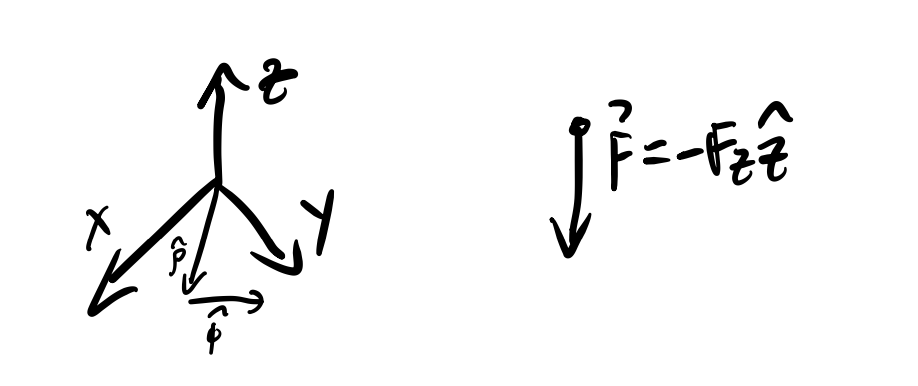
\includegraphics[scale=0.35]{Lectures/Images/lec12-coordinates.png}
\end{center}

What would a velocity field look like? Supposing $\v{F} = -F_z\zhat$, for the normal Stokeslet we have:
\begin{equation}
    \v{v}_0(\v{r}) = -\frac{F_z}{8\pi\mu r^3}\m{xz \\ yz \\ x^2 + y^2 + 2z^2}
\end{equation}
Looking at the magnitude of the velocity in the $xy$-plane (radial), we have:
\begin{equation}
    v^\rho_0(\v{r}) = \frac{xv_x + yv_y}{\sqrt{x^2 + y^2}} = -\frac{F_z}{8\pi \mu r^3}z\left(\frac{x^2 + y^2}{\sqrt{x^2 + y^2}}\right) = -\frac{F_z}{8\pi \mu r^3}z\rho
\end{equation}
and looking at the magnitude of the velocity in $\phi$ (tangential) we have:
\begin{equation}
    v^\phi_0(\v{r}) = \frac{-yv_x + xv_y}{\sqrt{x^2 + y^2}} = 0
\end{equation}

What about for the velocity arising from the odd viscosity? We find:
\begin{equation}
    \v{v}_\gamma(\v{r}) = \frac{\gamma}{8\pi \mu r^3}\m{yz \\ -xz \\ 0}
\end{equation}
where we find:
\begin{equation}
    v^\rho_\gamma(\v{r}) = 0
\end{equation}
\begin{equation}
    v^\phi_\gamma(\v{r}) = -\frac{\gamma F_z}{8\pi \mu r^3}\rho z
\end{equation}
So the leading order corrections to the velocity field due to odd viscosity are to induce some rotational/tangential flow!

\begin{center}
    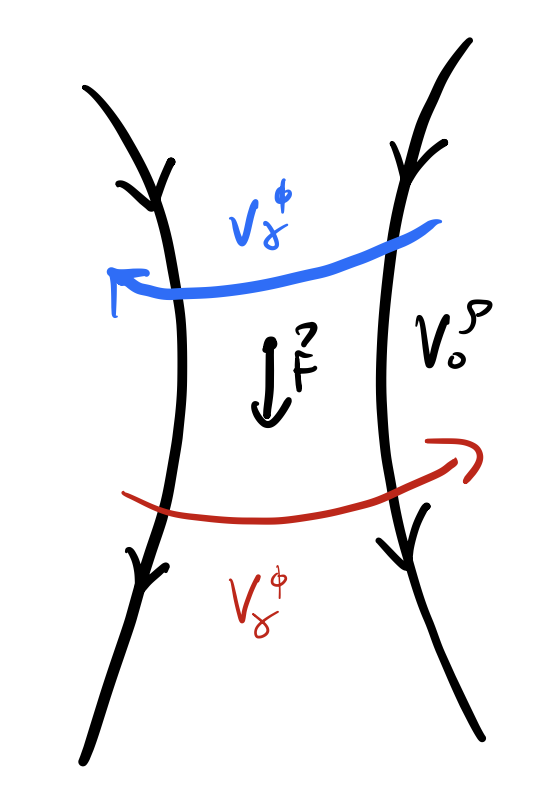
\includegraphics[scale=0.35]{Lectures/Images/lec12-velocityfield.png}
\end{center}

Note that we did the calculation perturbatively, but we are able to do the calculation for any $\gamma$. The flows in 3D look like:

\begin{center}
    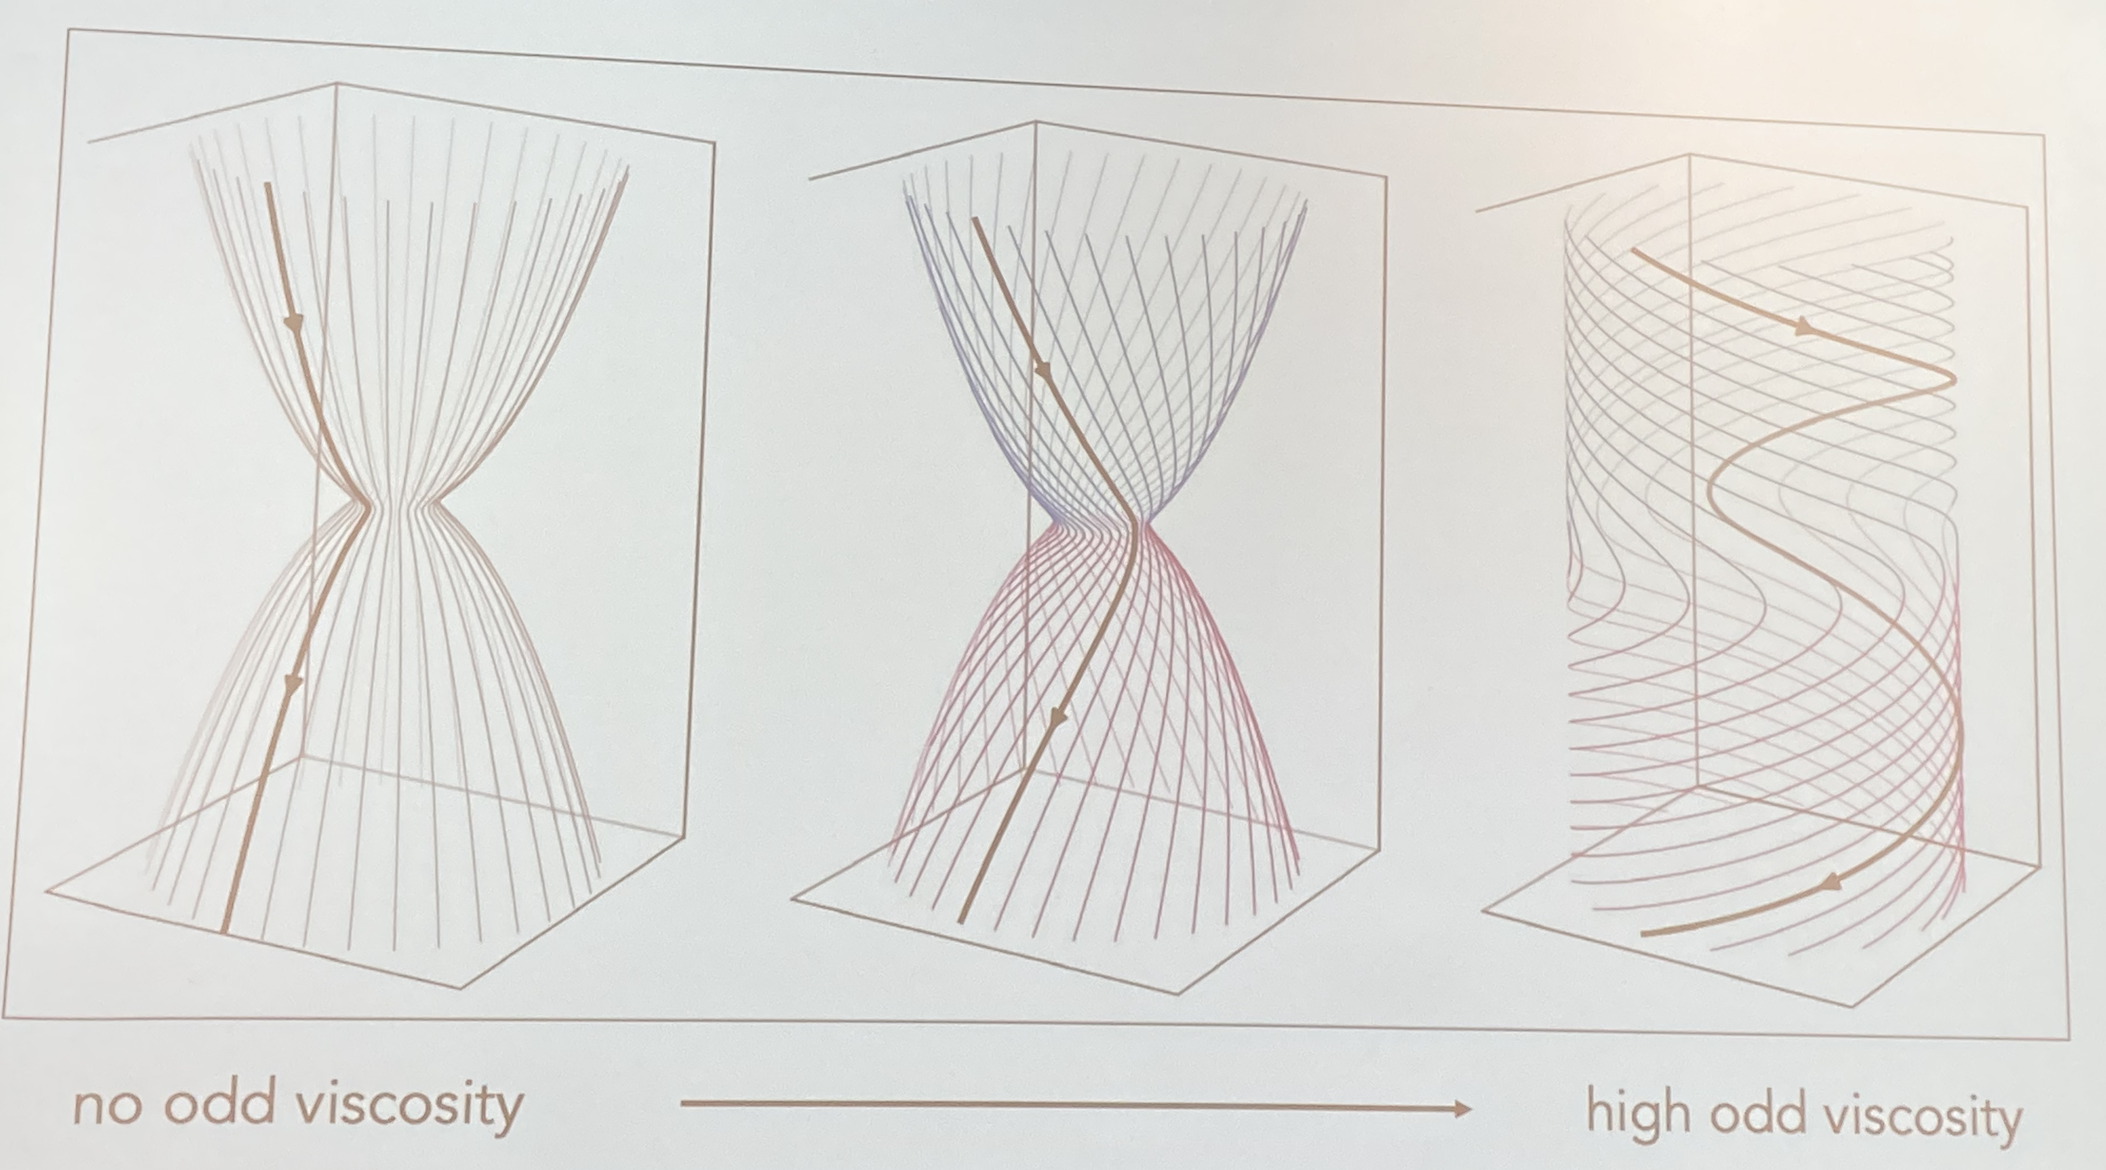
\includegraphics[scale=0.35]{Lectures/Images/lec12-velocityfieldstokeslet.png}
\end{center}

\subsection{Velocity Field with Sphere}
If we are interested in how the fluid moves past the sphere, we now have the correction (for the normal fluid case):
\begin{equation}
    \v{v} = \frac{\v{F}}{8\pi \mu}[1 + \frac{a^2}{6}\nabla^2]\mathbb{G}
\end{equation}
as in close to the sphere we are not able to neglect the $a^2$ term/treat it as small. The first order correction comes in the form of an azimuthal flow:
\begin{equation}
    v_\phi(r, z) = \frac{3aVrz(r^2 + z^2 - a^2)}{4(r^2 + z^2)^{5/2}}
\end{equation}

\begin{center}
    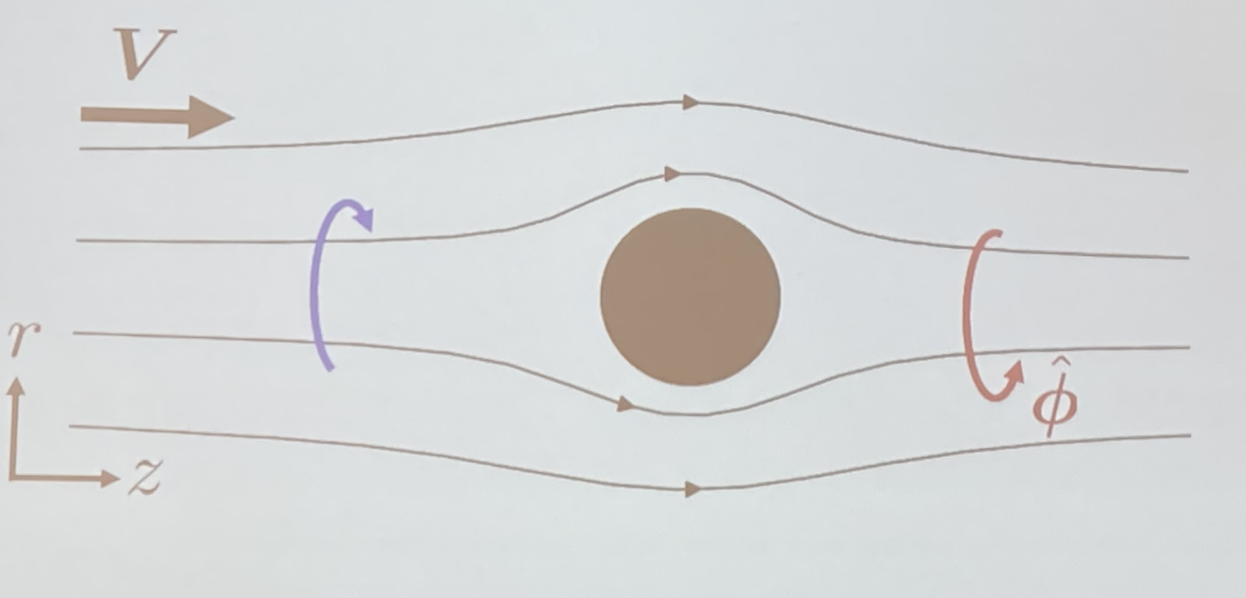
\includegraphics[scale=0.35]{Lectures/Images/lec12-oddsphere.png}
    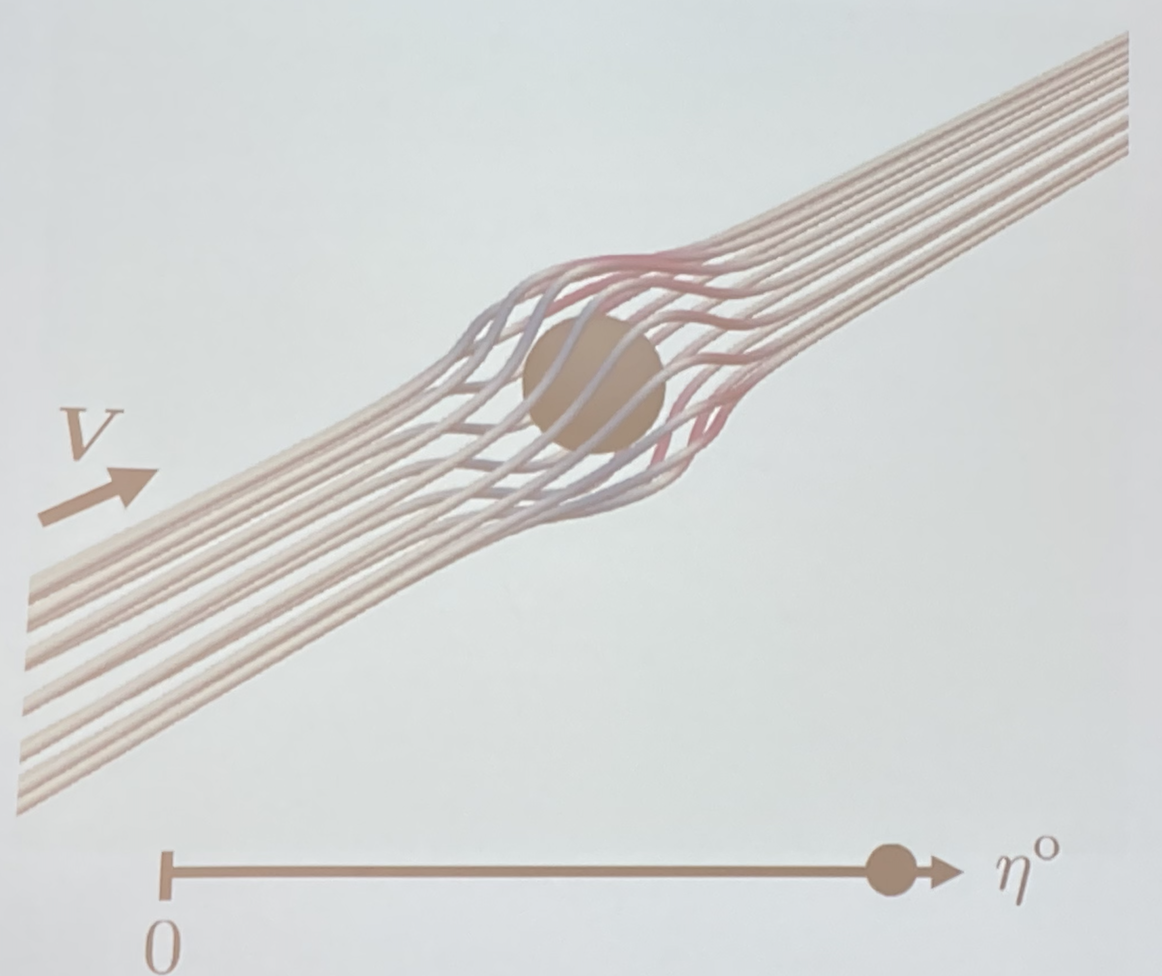
\includegraphics[scale=0.35]{Lectures/Images/lec12-oddsphere3d.png}
\end{center}

Also - odd viscosity in fluid causes velocity of sphere in a tilted direction (a ``lift force'') when an external force is applied; this is due to the asymmetric mobility matrix:
\begin{equation}
    \m{V_x \\ V_y \\ V_z} = \frac{1}{6\pi\mu a}\m{1 & \e/2 & 0 \\ -\e/2 & 1 & 0 \\ 0 & 0 & 1}\m{F_x \\ F_y \\ F_z}
\end{equation}

\begin{center}
    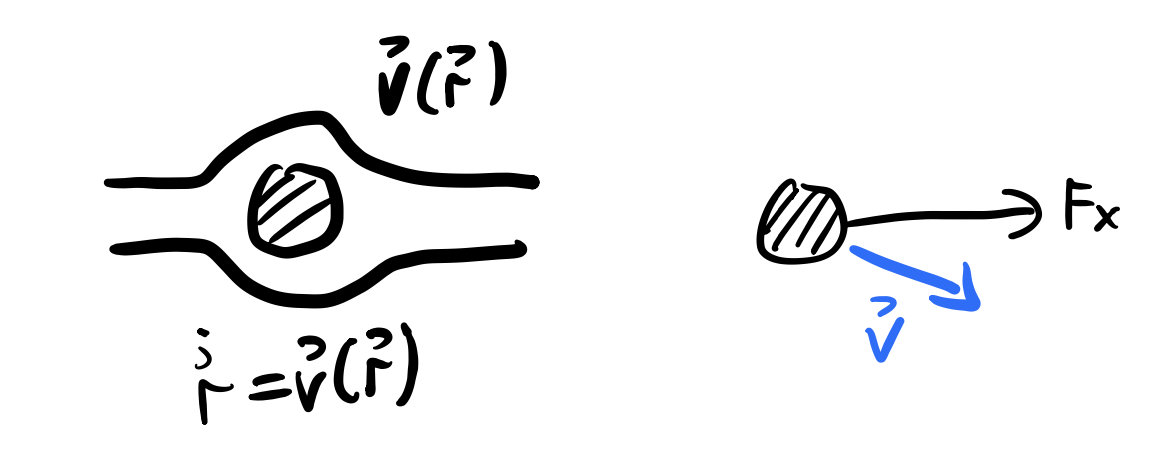
\includegraphics[scale=0.35]{Lectures/Images/lec12-liftforce.png}
\end{center}

Can also look at the many-body version of this problem (``many-body sedimentation''), wherein a cloud of such particles interact through the fluid. The particles in the cloud can display radial/tangential motion, and the competition between these two can change the shape of the cloud of particles (from toroidal to elliptical).